\documentclass[a4paper,14pt]{extarticle}

%%%%%%%%%%%%
% Preamble

% The most important
\usepackage{examstylo}
%%% Provides the following:
%% For typesetting
% \mrm{} % shorthand mathrm
% \thus % Implication symbol (=>)
% \sm % small minus (for \sm2 - 2 = \sm 4)
% \meuro % neat euro sign
% \deg % degree
% \mli{} % multiletter identifier (prevents linebreak)
% \cldots % compact \ldots
% \oldots % orange compact \ldots (like in Kern)
% \rom{} % roman numeral
% \intextbullet % Make a bulletpoint
% \lognl[base] % make a logarithm base base
% \deriv{y}{x} % make total derivative dy/dx
% \Xbar % Bar over X
% \hateq % = with ^ on top (for equivalent)
% \ut{} % for unit (is \,\mrm{#1})
% \eulere
% \cancel and \cancelto from the cancel package
%
%% For control
% \comment{} comment everything inside
%
%% And some colors
% \red{}
% \blue{}
% \orange{} % Like in Kern
% \royalpurple{} % Stolen from Wim, used in \answer

%%% Some notes:
% \newsubquestion{}{} works with package paracol to make two columns. if you want a newline after the subquestion, put the \newline INSIDE the question txt (i.e., {example text\newline}) 
% use \begin{multicols}{2} for two-column subquestions. its not perfect but so arent you
  % It will force an empty line above (and below?) use \vspace{-\lineheight} to remedy
% Watch out with a \footnote: margin notes do not move with the text to the newpage after a footnote was inserted.
% You can use \insertemptypage to insert an empty page



%%%%% %%%%% Options!
%% Uncomment this to use Arial (Ugly!)
\UseArialFont % < This


%% Footer options
\SetFooterOptions[% Set options for the footer
  showleft=False,%=True
  showcenter=True,%=True
  showright=True,%=True
  ]{}

%% Exercise options
\SetExerciseOptions[% Set options for exercises
  PutExerciseOnNewPage=False,%=True to show every (except first) exercise on a new page
  PutFirstExerciseOnNewPage=False,%=True to have the first exercise on a new page
  firstexercisevskip=\baselineskip,%=\baselineskip if first exercise not on new page, how much vspace before?
  QuestionStartingNumber=1,%=1 Start at question number #
  ]{}

%% Pages options
\SetPagesOptions[% Set options for the pages
  TitlePage=Simple,%=Simple [Make Simple Title], =Full [Make full title page], =False [No title]
  FormulaPage=False,%=False [No],=True [Yes]
  WorksheetPages=False,%=False [No],=True [Yes]
  ]{}
  
%% Worksheet options
\SetWorksheetOptions[% Set options for worksheet
  ShowTitle=False,%=True to show the title on the first page of the worksheets
  ]{}
  
%% Simple titlepage options
\SetSimpleTitleOptions[% Set options for simple title
  theStyle=Default,%=Default [Attempts to look like full titlepage, but small], =Exerciselike [Looks more like the exercise seperator]
  ]{}

%% Point options
\SetPointOptions[% Set options for points
  which=questions,%=questions [Use points from questions], =subquestions [Use points from subquestions], =False/None [No points]
  ]{}

%% Answer options
\SetAnswerOptions[% Set options for answers
  ShowAnswers=False,%=True [Show answers? global toggle]
  ShowAnswersInline=True,%=True [If show answers, show inline?]
  ShowAnswersAtEnd=False,%=True [If show answers, show at end?] % Currently doesnt work
  ]{}


%%%%% Title Page Settings
\title{Test for a test}
\extratitletext{{\Large Versie A}} % extra concise info e.g, {\Large Versie A}
%\leftfoottext{testtest-v0} % Text in the left box of the footer

%\date{30 Nov}
%\time{09:02\enspace--\enspace16:20\,uur}

\noteforthelastpage{% Put text here to have a note on the last page
%\textbf{Credit:} Hello this is credit which is shown on the last page.
} % end text for lastpage note

%%% Put text for the title page Here
% Use \totqstns and \totpts to reference total questions and total points resp.
\titlepagetext{
Bij dit examen hoort een uitwerkbijlage. 

\vfill
Dit examen bestaat uit \totqstns\ vragen.\par
Voor dit examen zijn maximaal \totpts\ punten te behalen.\par
} % End of the title page text

%%% Put text here for the simple title on the first page
% Use \totqstns and \totpts to reference total questions and total points resp.
\simpletitletext{
\textit{Deze toets bestaat uit \totqstns\ vragen (\totpts\ punten).\\
Veel succes en plezier!\\
  }
}

%%%%% Formula Page (?)

\formulapagetext{% Put text here for the formula page(s)

\textsc{Overzicht formules}\\

\textbf{Differenti\"eren}\\[0.5\baselineskip]\noindent
\begin{tabular}{lll}
\hline\hline
Naam van de regel & Functie & Afgeleide \\\hline
somregel & $s(x) = f(x)+g(x)$ & $s'(x) = f'(x) + g'(x)$ \\
verschilregel & $v(x) = f(x)-g(x)$ & $v'(x) = f'(x) - g'(x)$ \\
productregel & $p(x) = f(x)\cdot g(x)$ & $p'(x) = f'(x)\cdot g(x) + f(x)\cdot g'(x)$ \\
quoti\"entregel & $q(x) = \frac{f(x)}{g(x)}$ & $q'(x) = \frac{f'(x)\cdot g(x) - f(x)\cdot g'(x)}{(g(x))^2}$ \\
kettingregel & $k(x) = f(g(x))$ & $k'(x) = f'(g(x))\cdot g'(x)$ of  $\deriv{k}{x} = \deriv{f}{g}\cdot\deriv{g}{x}$ \\
\hline
\end{tabular}\newline

\textbf{Logaritmen}\\[0.5\baselineskip]\noindent
\begin{tabular}{ll}
\hline\hline
Regel & Voorwaarde \\\hline
$\lognl[g] a + \lognl[g] b = \lognl[g] ab$ & $g>0,\ g\neq1,\ a>0,\ b>0$\\
$\lognl[g] a - \lognl[g] b = \lognl[g] \frac{a}{b}$ & $g>0,\ g\neq1,\ a>0,\ b>0$\\
$\lognl[g] a^p = p\cdot\lognl[g] a$ & $g>0,\ g\neq1,\ a>0$\\
$\lognl[g] a = \frac{\lognl[p] a}{\lognl[p] g}$ & $g>0,\ g\neq1,\ a>0,\ p>0,\ p\neq 1$\\

\hline
\end{tabular}

} % End of formula page text

%%%%% HACKZ
\setlength{\exerciseskip}{2\baselineskip} % for use in \interexercisespace
\def\arraystretch{1}%  1 is the default, change whatever you need % Table row sep
  
%%%%% Examples
% Wrapfigure
%\begin{wrapfigure}[]{r}{0.3\textwidth} % Use for illustrations, not figures
%\begin{wrapfigure}[<number of lines>]{<capital for float>}{0.5\textwidth}
%\centering
%    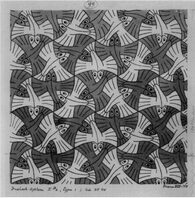
\includegraphics[width=0.25\textwidth]{escher.jpg}
% \caption{}
%\end{wrapfigure}

% Answer
% \answer[<before>][<after>]{answer}
% is only shown when showanswers=True. <before> and <after> are only printed inline

%%%%% %%%%% BEGIN document
\begin{document}

%%% New exercise
%\newexercise{Lorem} \label{exc:lorem}



%\interexercisespace


\newquestion[3]{\label{q:vraagX}quis nostrud exercitation ullamco laboris nisi ut aliquip ex ea commodo consequat. ea commodo consequat.} 
\newsubquestion[2]{No sabía, de tristezas, ni de lágrimas, Ni nada, que me hicieran llorar,}
\answer{\begin{bolletjes}
  \bolletje Que a besos yo te levante al rayar el día
\end{bolletjes}}
\newsubquestion[2]{Yo sabía de cariño, de ternura. Porque a mí desde pequeño Eso me enseño mamá,}
\answer{\begin{bolletjes}
  \bolletje Y que el idilio perdure siempre al llegar la noche
\end{bolletjes}}
\newsubquestion[2]{eso me enseño mamá Eso y muchas cosas más.}
\answer{\begin{bolletjes}
  \bolletje Y cuando venga la aurora llena de goce
\end{bolletjes}}
\newsubquestion[2]{Yo jamás sufrí, yo jamás lloré. Yo era muy feliz, yo vivía muy bien\newline}
\answer[\undonewline]{\begin{bolletjes}
  \bolletje Se fundan en una sola tu alma y la mía
\end{bolletjes}}

\showpoints
\newquestion[3]{\label{q:vraagXX}quis nostrud exercitation ullamco laboris nisi ut aliquip ex ea commodo consequat. En quaestio~\ref{q:vraagXXX} habes responsum.\newline} 

\answer[\undonewline]{\begin{bolletjes}
  \bolletje Ceterum censeo Carthaginem esse delendam
  \bolletje Heldhaftig, vastberaden en barmhartig
\end{bolletjes}
Opmerking: \textit{Abundat dulcibus vitiis}}

\newquestion[3]{\label{q:vraagXXX}quis nostrud exercitation ullamco laboris nisi ut aliquip ex ea commodo consequat. ea commodo consequat.}\vspace{-\lineheight}%\vspace{-0.83333\baselineskip}  
\begin{multicols}{2}%
\newsubquestion[2]{$y=x^2-3$}
\newsubquestion[2]{$L=4\pi R^2 \sigma T^4$}
%\newsubquestion[2]{$y=x^2-3$}
\newsubquestion[2]{\label{sq:subq}Yo jamás sufrí, yo jamás lloré. Yo era muy feliz, yo vivía muy bien}
\columnbreak% Notice the columnbreak
\newsubquestion[2]{$y=x^2-3$}
\newsubquestion[2]{$y=x^2-3$}
\newsubquestion[2]{$y=x^2-3$}
\end{multicols}



%%% This is the end (do not touch)
\lastpageofthetest\
%%

%%%%% HERE STARTS THE WORKSHEETS
\worksheetcontent{ % Put content here for the worksheets
                   % Use \refquestion{<label>} to refer to a question
\refquestion{q:vraag}\newline
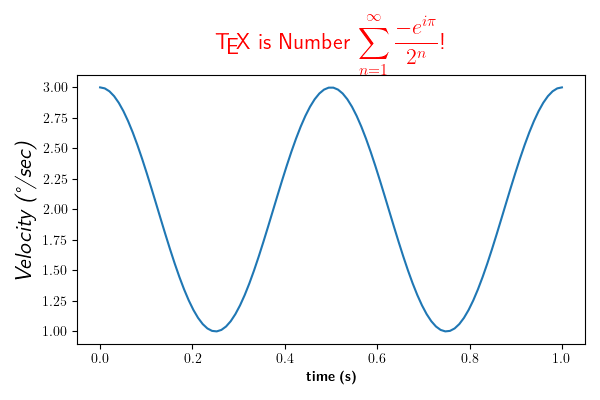
\includegraphics[width=0.8\textwidth]{random_graph.png}

\vfill

\refquestion{q:vraagvier}\newline
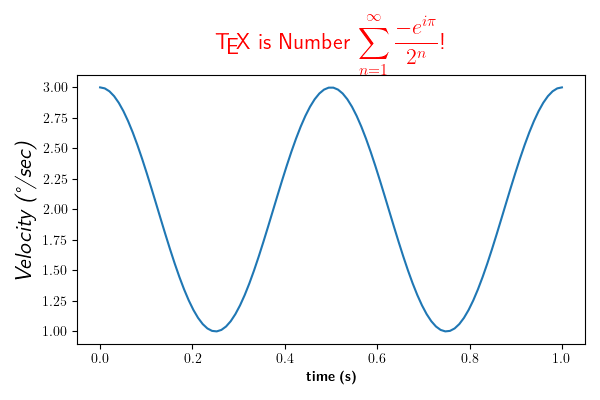
\includegraphics[width=0.8\textwidth]{random_graph.png}

\newpage

\refquestion{q:vraagvijf} en \refquestion{q:vraagzes}\newline
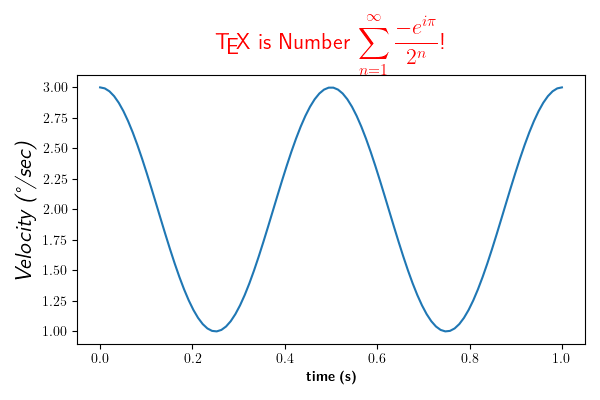
\includegraphics[angle=90,width=0.8\textwidth]{random_graph.png} % Sidenote: The rotating package introduces a sidewaysfigure

%\vfill
%\begin{center} \textbf{\textsc{VERGEET NIET DEZE UITWERKBIJLAGE IN TE LEVEREN}} \end{center}

} % End worksheet content


%%% END Document
% It makes the worksheets here
\end{document}
